\documentclass{article} % For LaTeX2e
\usepackage{cos424,times}
\usepackage{hyperref}
\usepackage{url}
\usepackage{graphicx}
\usepackage{amsmath}
\usepackage{multirow}
\usepackage{wrapfig}
\usepackage[
backend=biber,
style=numeric,
sorting=ynt
]{biblatex}
\providecommand{\tabularnewline}{\\}
\usepackage{array}
\usepackage{booktabs}
\usepackage{setspace}



\addbibresource{ref.bib}
\title{Value of names in a namespace}


\author{
Paul Ellenbogen \\
Department of Computer Science\\
Princeton University\\
\texttt{pe5@princeton.edu} \\
\And
Miles Carlsten\\
Department of Computer Science \\
Princeton University\\
\texttt{carlsten@cs.princeton.edu} \\
\And
Harry Kalodner\\
Department of Computer Science \\
Princeton University\\
\texttt{kalodner@cs.princeton.edu} \\
}

\newcommand{\fix}{\marginpar{FIX}}
\newcommand{\new}{\marginpar{NEW}}

\begin{document}

\maketitle

\begin{abstract}
\end{abstract}

\section{Introduction}
    Our research project focuses on trying to predict the value of a given name in the Namecoin DNS namespace. We want to be able to identify which features make different names in this space more valuable than others. Like Bitcoin, all transactions that have ever happened in the Namecoin ecosystem are recorded and are publicly available, which is great for data analysis. In order to motivate this project, we must first give a background on Namecoin. We will then motivate the project, describing the namespace. We also describe how we attribute value to a name. 

\subsection{Background on Namecoin}
    Namecoin is an alternative cryptocurrency that is closely related to Bitcoin. Namecoin was the first 'altcoin' in the sense that it was the first alternative cryptocurreny to run its own blockchain alongside Bitcoin's. Namecoin is almost identical to Bitcoin except that Namecoin also provides easy tools for using the blockchain as an arbitrary key/value (we will refer to these as name/value) datastore. Because Namecoin is so similar to Bitcoin, it is necessary to briefly mention some of the features of Bitcoin that Namecoin shares. Bitcoin is a decentralized consensus based cryptocurrency. Bitcoin uses an append-only log, called the blockchain, in order to keep track of all the transactions between the users of the system. A user of Bitcoin will own an address that is able to sign transactions authorizing the exchange of coins. In order to add transactions to the blockchain, a user must present the solution to a computationally difficult cryptopuzzle. The users who actively try to solve this puzzle and add transactions to the blockchain are known as Bitcoin miners. Most users are not miners, but the miners will include other user's transactions when they add to the blockhain because users will typically add a small tip to the miners on the transactions. The security of the blockchain is guaranteed by 'proof of work' that someone must present to add to the blockchain. As long as the majority of miners (weighted by computational power) are not malicious, a malicious user will not be able to corrupt the blockchain. Namecoin is merge mined with Bitcoin, so it enjoys a high difficulty from the proof of work challenge because there are many large Bitcoin mining pools that also mine Namecoin in parallel {ref: something on merge mining?}. For a more thorough description of the details of Bitcoin, see {ref satoshi}.
    
    Namecoin offers all of the same features as Bitcoin, supporting the same number of coins, the same block creation time, and the same cryptographic puzzle format. The additional feature of Namecoin is that it allows users to store name/value pairs in the blockchain where a user is able to register a particular value to a name. The name is associated with a Namecoin token which can be traded amongst users of the system. Whoever owns the token can change the value associated with the name. One of the first suggested uses of Namecoin was to replace modern DNS\footnote{The reason there is interest in a service like this is because a blockchain based DNS has potential advantages over ICANN DNS. As a specific example, because the blockchain is decentralized, no central authority can arbitrarily censor any domain.}. In the new system, a domain would be a name that a user would own on the Namecoin blockchain. The owner can then set the associated value to whatever they need in order to point browsers supporting Namecoin DNS to the correct destination. This name/value store has many uses beyond a new DNS system, but that is beyond the scope of this paper, and our machine learning techniques will only apply to the names used in the DNS system running on Namecoin. We will quickly cover the features in Namecoin that allow for this new functionality and then walk through an example of how it's used. 

    The difference between Bitcoin and Namecoin happens inside the scripting language used to create the transactions. There are several different commands in the scripting language that can be used to make a transaction, but only a subset are accepted by most miners. In Namecoin, a few new commands are added to the scripting language. The new commands don't add any new functionality to the transactions themselves, but they do act as a marker for data that is worked into the transaction script. The data that these signals proceed is the data that is used in the Namecoin protocol. There are three new script operations in Namecoin: NAME\_NEW, NAME\_FIRSTUPDATE, and NAME\_UPDATE. 

\begin{figure}
\begin{centering}
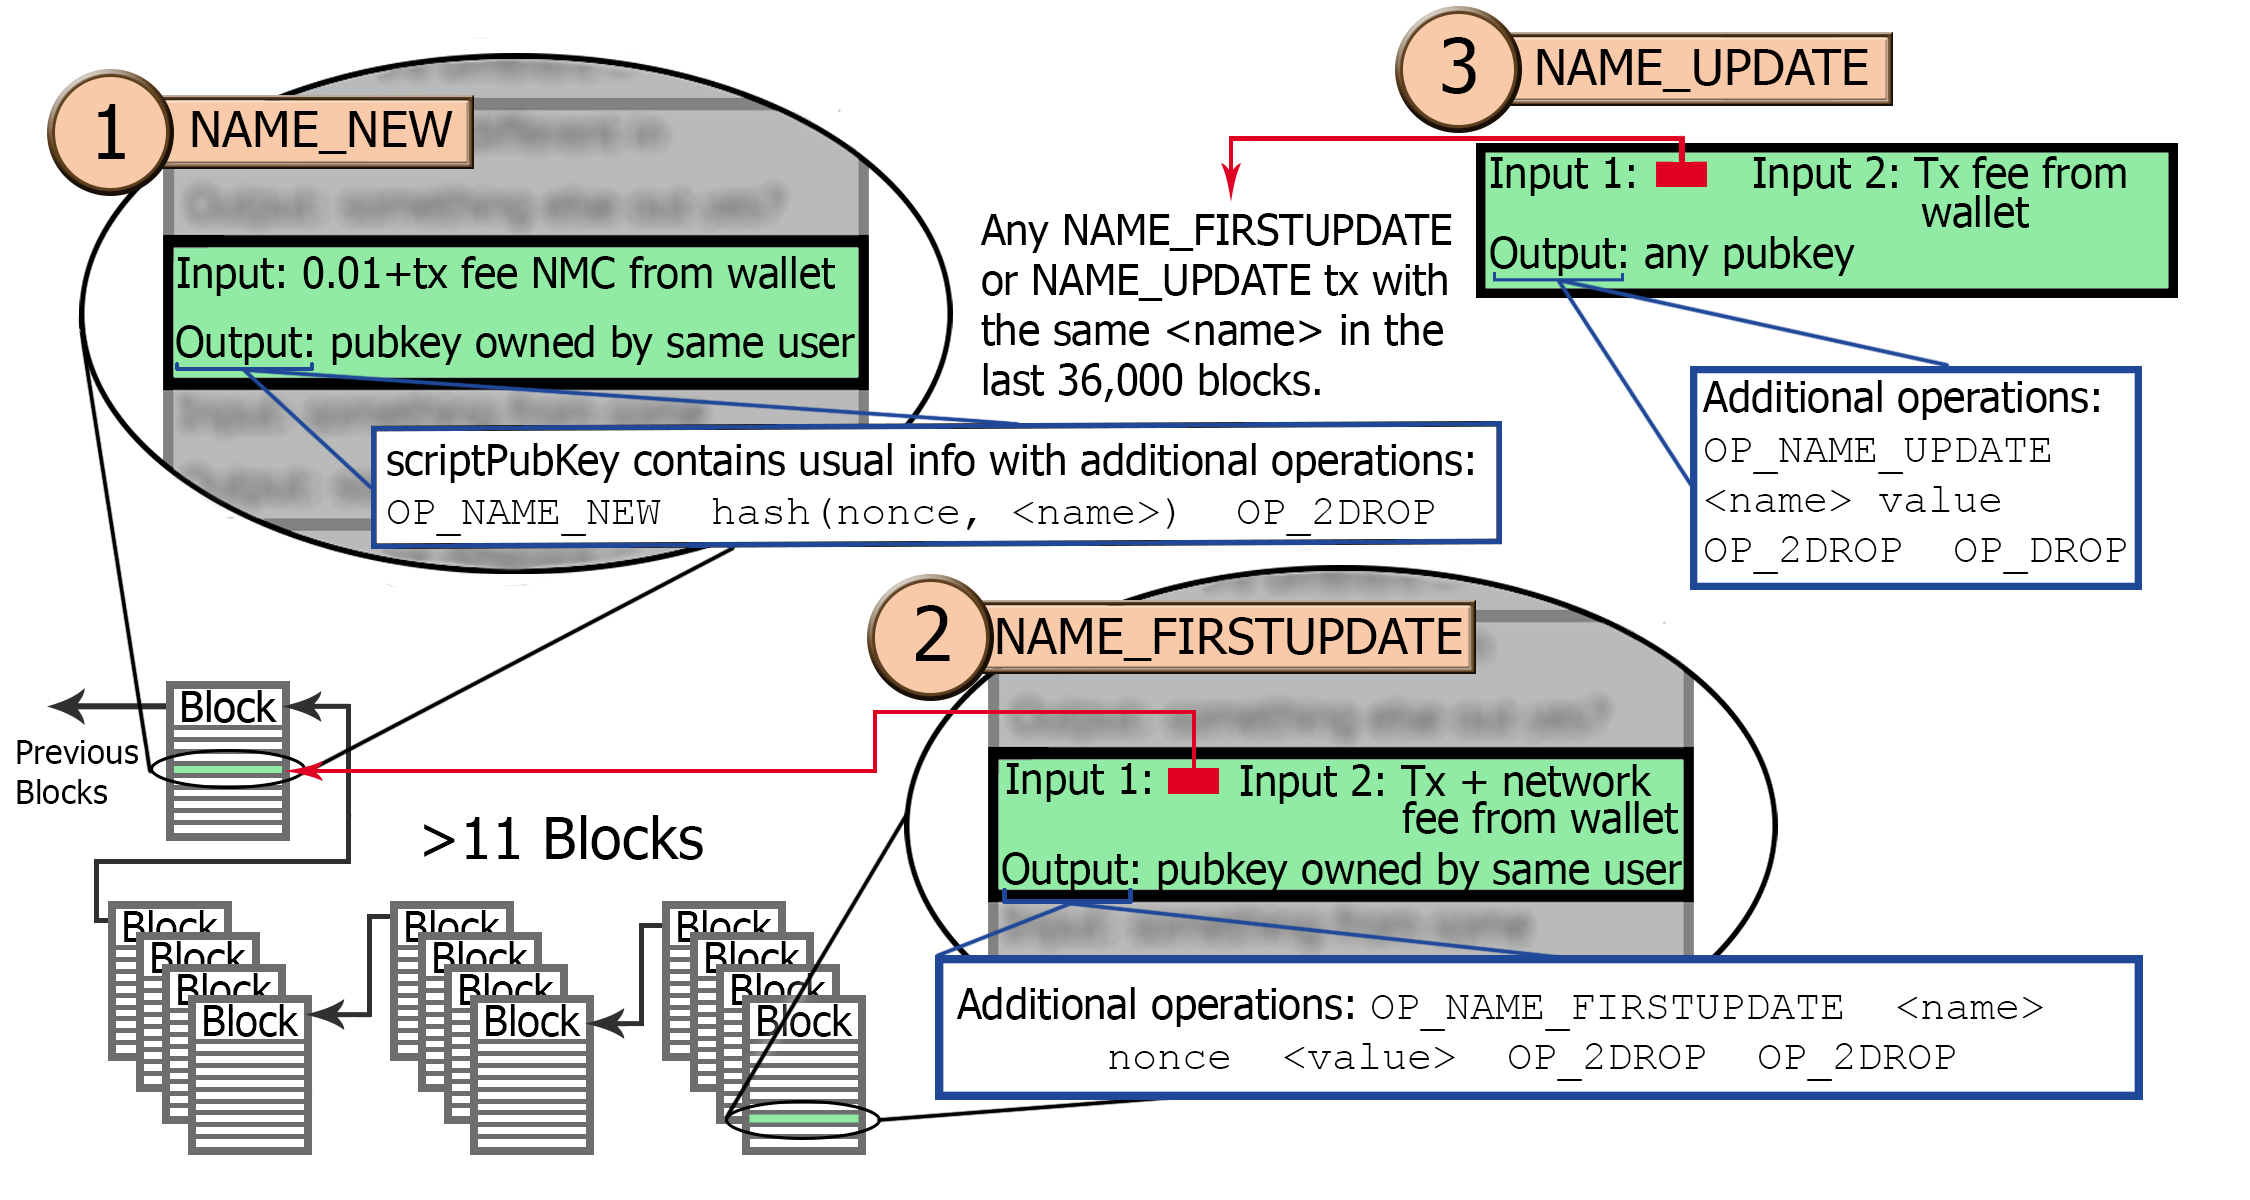
\includegraphics[scale=0.8]{registration}
\par\end{centering}
\protect\caption{Diagram indicating the transactions and script operations involved in registering a name in the Namecoin system. \label{fig:registration}}
\end{figure}

    We will now walk through a simple example of a user trying to register a name in the Namecoin system, following what is seen in figure \ref{fig:registration}. Say a user is interested in registering the domain example.bit. The first step is for the user to create a special transaction using the NAME\_NEW script operation. The data that they will push onto the blockchain will be a hash of a concatenation of the name that they want to register (example) and a random nonce. They will then need to wait for a period of at least 12 blocks before they can then create the next special transaction. They will now create a transaction containing the NAME\_FIRSTUPDATE operation, citing the previous NAME\_NEW transaction as input. This transaction requires them to push data that shows the name and random nonce used in the NAME\_NEW transaction and allows them to set the first value associated with example.bit. The reason that the NAME\_NEW transaction is needed at all has to do with preventing front running, where another user hears the transaction claiming a name and tries to claim the name first and then sell it to the original user. Finally, whenever a user wants, they can now create a transaction that utilizes the final script operation, NAME\_UPDATE. When they make a NAME\_UPDATE transaction, they will cite an output of a NAME\_FIRSTUPDATE or NAME\_UPDATE transaction that they made as input and indicate a new value for that transaction to take. If a name on the blockchain has not been in a NAME\_FIRSTUPDATE or NAME\_UPDATE transaction in the past 36,000 blocks, then the name is considered expired and it is available again for any user to claim with a NAME\_NEW transaction. For more details about the specifics on how Namecoin works, see {ref US!!!!}.

\subsection{Motivation and goal}

    A major issue that Namecoin faces is that it is filled with squatters. Any user can claim a name if they are willing to pay the small associated fees (see {ref us}). A squatter's goal is to claim names that have the most value; a squatter wants to claim names that they will be able to trade to others for the most. The motivation of this research is to figure out which features (which we will discuss in detail later) make a name more valuable. In ideal situation, we would like to train our machine learning algorithms using the sale prices of names from squatters to users of the system, but unfortunately, this is not possible. We have carefully looked for evidence of transfers of domain names from squatters to normal users, but have found that these events are rare. In order to calculate the value of a name, we must use other indicators to determine the value of a name. There are several indicators that we use instead to judge a name's value.

{\bf Whether a name has been claimed.} The most important indicator of a name's value to a squatter is whether or not the name has been claimed at all by any squatter. The unfortunate part of this is that it is binary-- all names have either been claimed by a squatter, or they have not. Of the names that have not been claimed, there are no more blockchain features we can use to predict value, because they will not appear on the blockchain. On the other hand, names that have been claimed have additional indicators that can signal value.

{\bf Length of time registered.} The longer a name has been registered can indicate that squatters think a name is more valuable. If a name has been registered for a long period of time, it means that a squatter (or squatters) have taken enough interest in a name in order to go to the effort of paying for update transactions to not let a name expire. 

{\bf Time a name was first registered.} The cost to claim a name was initially much higher (as a deterrent to initial squatters) than it is now. The names that squatters grabbed early on cost the squatters a lot more than names that they picked up later in the life of Namecoin. 

{\bf Resurrection gap.} When a name has not been updated for 36,000 blocks, it becomes dead and can be claimed by any user with a NAME\_NEW transaction. If a name is immediately resurrected after it expires, then it is more valuable than a name that stayed dead indefinitely, or stayed dead for a longer period before resurrection. 



\section{Methods}
 
\section{Analysis}


\section{Conclusion}

\newpage
\printbibliography

\end{document}


